% !TEX root = 1_power_supply.tex
\documentclass[1_power_supply.tex]{subfiles}
\graphicspath{{../figures/}}
\begin{document}

\section{太陽電池の特性}

\subsection{目的}

\begin{enumerate}
	\item 照度と,光源からの距離との関係を調べる.
	\item 太陽電池の特性を測定し,等価回路のパラメータや出力できる電力について評価する.
\end{enumerate}

\subsection{原理}

今回作成するシステムの入口となる光エネルギーから電気エネルギーへの変換部分を担うのが太陽電池であり,これは,ダイオードの光特性を利用した素子である.太陽電池の等価回路は図\ref{fig:1_2}の青点線部で表される.このとき図\ref{fig:1_2}中の$V,I$に関して,
\begin{align}
	I = I_\mathrm{ph}-I_0\left\{\exp[\frac{e(V+R_\mathrm{s}I)}{nkT}-1]\right\}-\frac{V+R_\mathrm{s}I}{R_\mathrm{sh}}
\end{align}

という関係が成り立つ.ここで,$I_0$ :飽和電流,$e$ :電気素量,$k$ :ボルツマン定数,$n$ :接合定数,$T$ :絶対温度,$I_\mathrm{ph}$ :光電流である.

\begin{figure}[htbp]
	\begin{center}
		\scalebox{0.1}{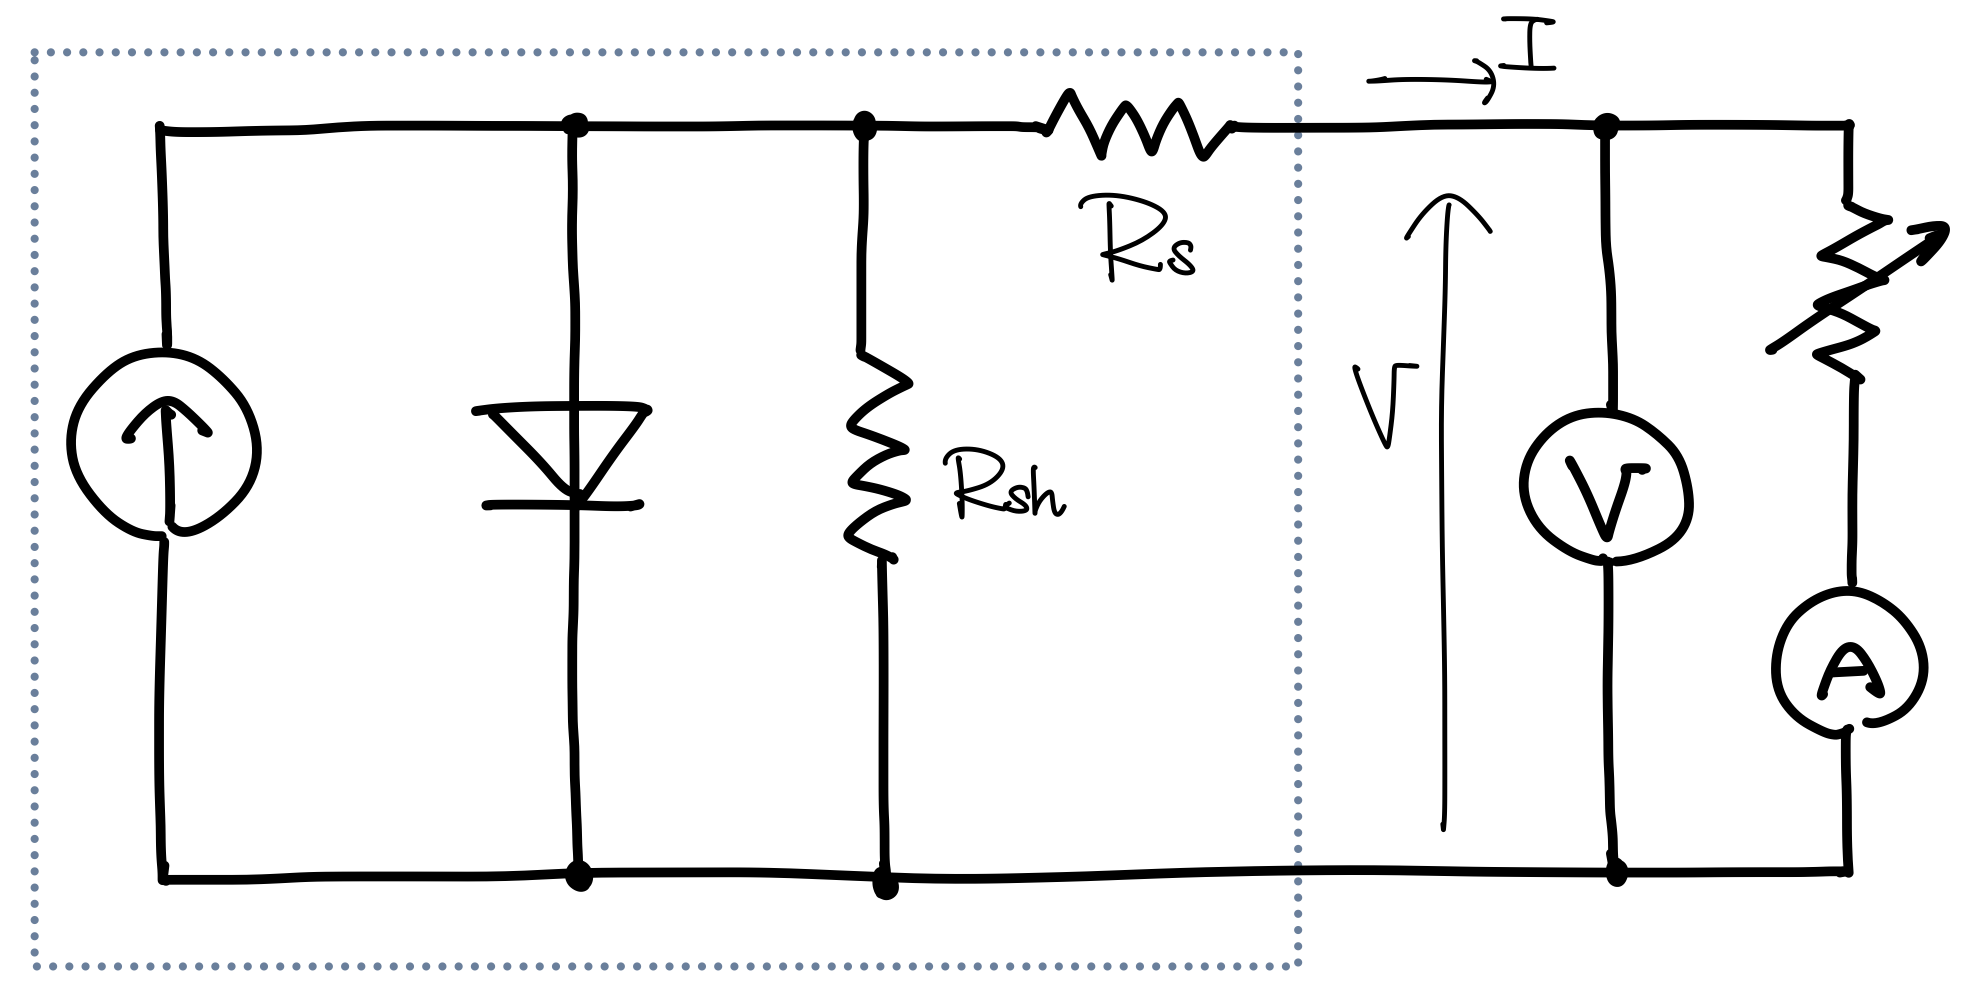
\includegraphics{1_2.png}}
		\caption{太陽電池の特性を測定するための回路}\label{fig:1_2}
	\end{center}
\end{figure}

等価回路の抵抗を求める際は,ダイオードが動作している(電圧源とみなせる)ときと,動作していない(開放とみなせる)ときに分けて考える.

\subsubsection{ダイオードが動作しているとき}

ダイオードの動作電圧を$V_\mathrm{on}$とすると,キルヒホッフの電圧則から,

\begin{align}
	V_\mathrm{on} = V+R_\mathrm{s}I
\end{align}

両辺を$V$で微分して,

\begin{align}
	0            & = 1+R_\mathrm{s}\dv{I}{V}                                       \\
	R_\mathrm{s} & = \left.- \dv{V}{I}\right|_{V\sim V_\mathrm{on}} \label{eq:R_s}
\end{align}

となる.

\subsubsection{ダイオードが動作していないとき}

キルヒホッフの電圧則から,

\begin{align}
	V+R_\mathrm{s}I = R_\mathrm{sh}(I_\mathrm{ph}-I)
\end{align}

両辺を$I$で微分して,

\begin{align}
	\dv{V}{I}+R_\mathrm{s} & = -R_\mathrm{sh}                                                 \\
	R_\mathrm{sh}          & = \left.-\dv{V}{I}\right|_{V\sim 0}-R_\mathrm{s} \label{eq:R_sh}
\end{align}

\subsection{方法}

\subsubsection{照度と光源からの距離に関する実験(実験1.1)}

\begin{figure}[htbp]
	\begin{center}
		\scalebox{0.2}{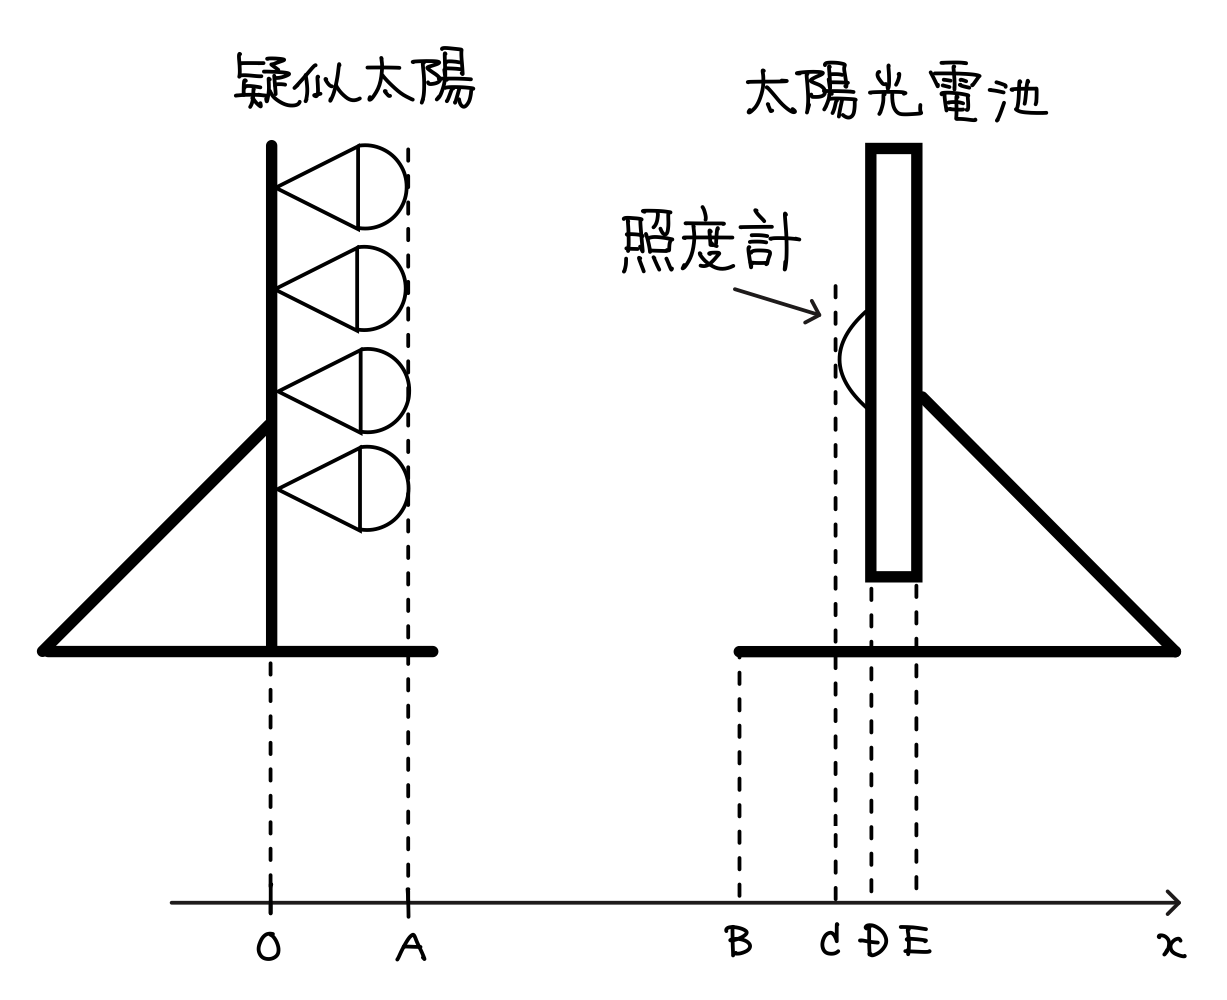
\includegraphics{1_1.png}}
		\caption{照度測定の様子を横から見た図}\label{fig:1_1}
	\end{center}
\end{figure}

図\ref{fig:1_1}のように擬似太陽と太陽光電池,照度計を配置し,疑似太陽と太陽光電池との間隔を変えて,太陽光電池の中央での照度を計測した.測定点は$\mathrm{OB}=\SIs{60}{\centi\meter},\SIs{75}{\centi\meter},\SIs{90}{\centi\meter},\SIs{105}{\centi\meter},\SIs{120}{\centi\meter}$の5点とした.
% なお,距離の測定は図\ref{fig:1_1}中OB間で行い,適切な変換でもってAC間の距離を導出した.測定した間隔は,OB間が$\SIs{60}{\centi\meter},\SIs{75}{\centi\meter},\SIs{90}{\centi\meter},\SIs{105}{\centi\meter},\SIs{120}{\centi\meter}$の5つの場合である.

\subsubsection{太陽電池の特性を調べる実験(実験1.2)}

\begin{figure}[htbp]
	\begin{center}
		\scalebox{0.11}{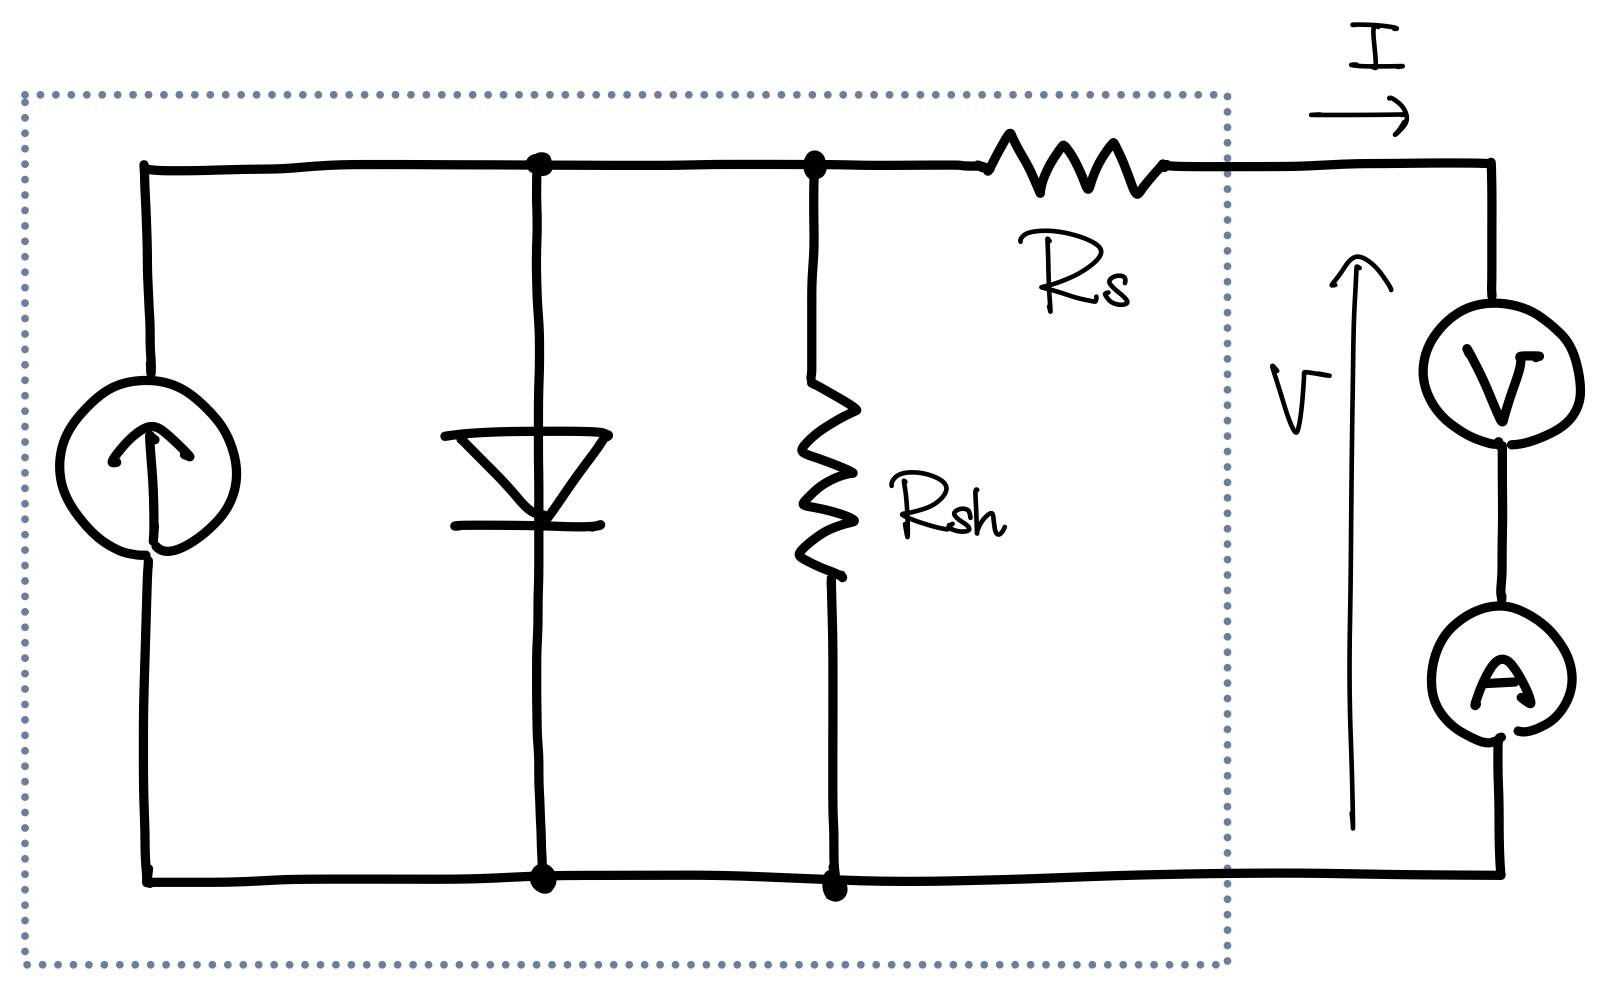
\includegraphics{1_3.png}}
		\caption{太陽電池の特性を測定するための回路($I$が$\SIs{0}{\ampere}$近傍のとき)}\label{fig:1_3}
	\end{center}
\end{figure}

図\ref{fig:1_1}中OB間の距離が$\SIs{60}{\centi\meter},\SIs{105}{\centi\meter},\SIs{120}{\centi\meter}$の3つの場合について,図\ref{fig:1_2}の回路を用いて$V,I$を測定した.また,$I$が$\SIs{0}{\ampere}$近傍の測定については,抵抗を印加しない開放での測定を再現するため,図\ref{fig:1_3}の回路を用いた.

\subsection{使用器具}
(型番を記していない器具については確認し次第追記します.)
\begin{enumerate}
	\item 太陽電池モジュール : 昭和ソーラーエネルギー(株) GT234
	\item 電圧計
	\item 電流計
\end{enumerate}

\subsection{結果}

\subsubsection{実験1.1}

$\mathrm{AC}=\mathrm{OB}-\SIs{4.5}{\centi\meter}$と照度の測定結果を図\ref{fig:1_dE}に示す.

\begin{figure}[htbp]
	\begin{center}
		\scalebox{0.5}{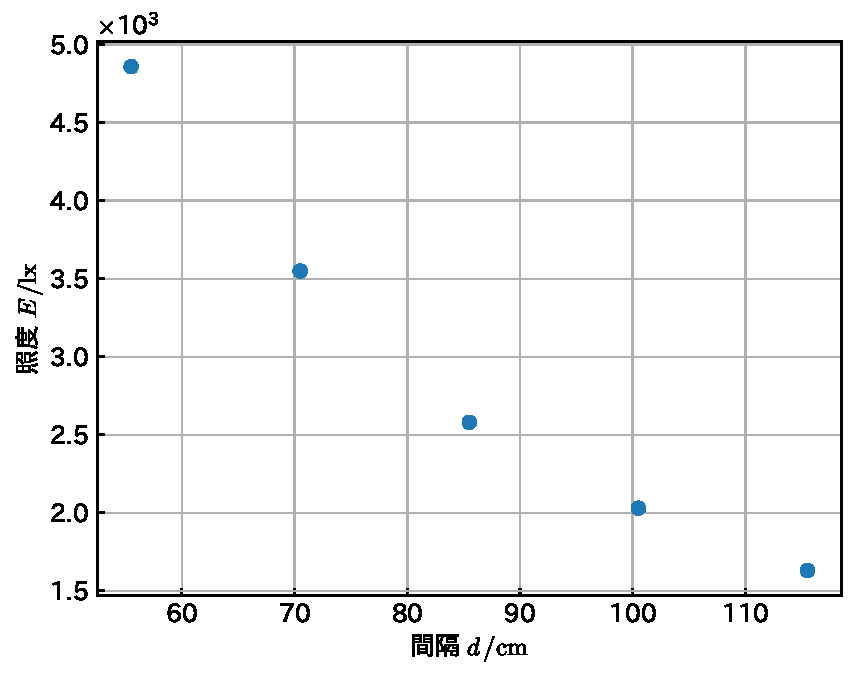
\includegraphics{1_dE.pdf}}
		\caption{光源から照度計までの距離と照度との関係}\label{fig:1_dE}
	\end{center}
\end{figure}

\subsubsection{実験1.2}

各間隔での電流電圧特性の測定結果を図\ref{fig:1_VI}に示す.

\begin{figure}[htbp]
	\begin{center}
		\scalebox{0.75}{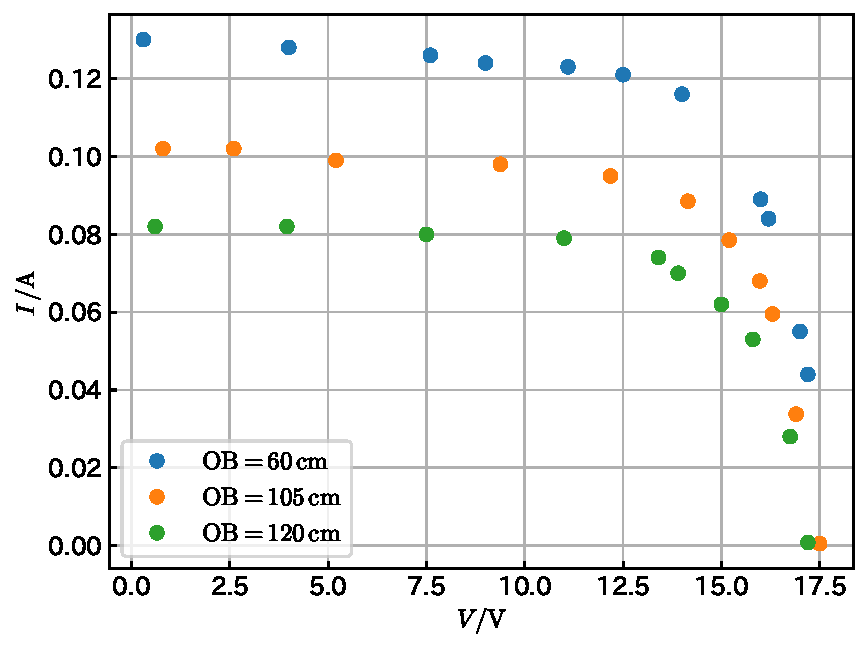
\includegraphics{1_VI.pdf}}
		\caption{光を照射したときの太陽電池の電流電圧特性の測定結果}\label{fig:1_VI}
	\end{center}
\end{figure}

\subsection{考察}

\subsubsection{実験1.1}

光源が点光源の場合は,照度は距離の逆二乗に比例することが知られている.今回の実験では点光源ではないことを考慮し,照度を$E$,距離を$d$とおいて,

\begin{align}
	E = \frac{A}{ad^2+bd+c}
\end{align}

に従うことを仮定する.$A,a,b,c$は定数である.図\ref{fig:1_dE}に対しフィッティングを行ったものを図\ref{fig:1_dE_fit}に示す.

\begin{figure}[htbp]
	\begin{center}
		\scalebox{0.5}{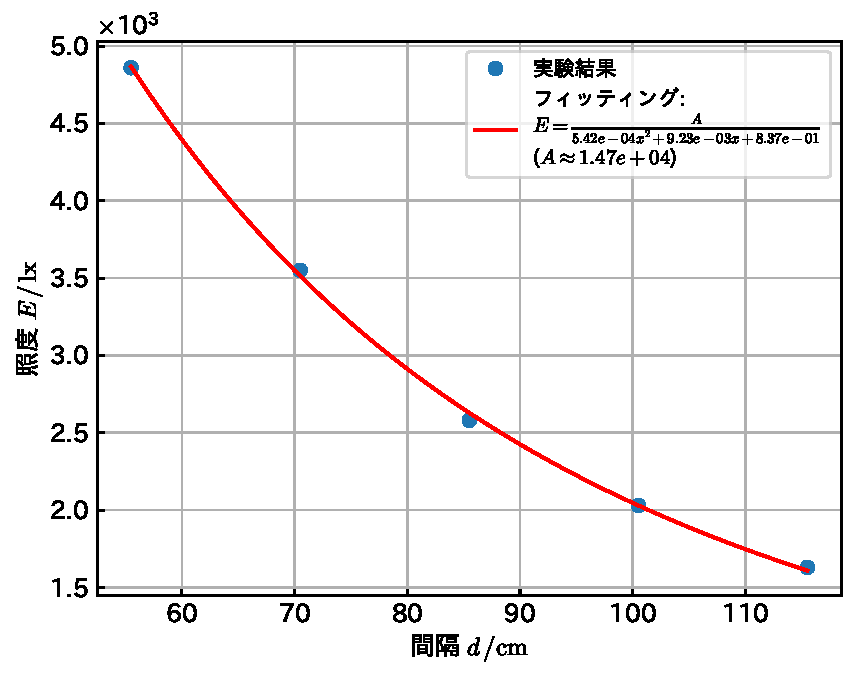
\includegraphics{1_dE_fit.pdf}}
		\caption{照度測定結果とそのフィッティング}\label{fig:1_dE_fit}
	\end{center}
\end{figure}

今回の測定から,

\begin{align}
	E = \frac{\SIs{1.47e4}{\lumen}}{(\num{5.4e-4})\times d^2+(\SIs{9.2e-3}{\meter})\times d+(\SIs{0.84}{\meter^2})}
\end{align}

と係数を決定できた.

\subsubsection{実験1.2}

代表として$\mathrm{OB}=\SIs{105}{\centi\meter}$の場合について解析する.

\begin{figure}[htbp]
	\begin{center}
		\scalebox{0.5}{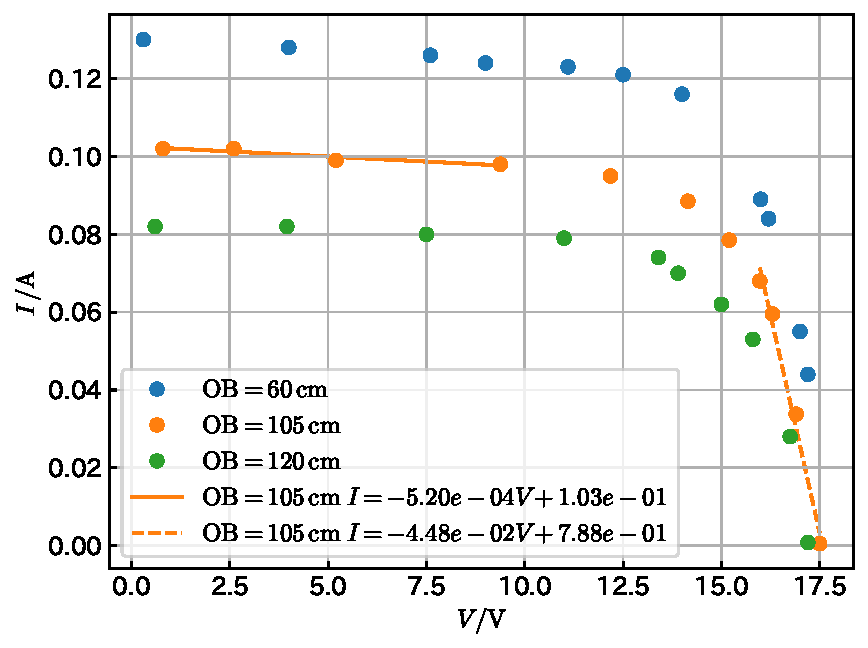
\includegraphics{1_VI_fit.pdf}}
		\caption{電流電圧特性の測定結果とフィッティング}\label{fig:1_VI_fit}
	\end{center}
\end{figure}

ダイオードが動作している領域・動作していない領域でフィッティングした図を図\ref{fig:1_VI_fit}に示す.ここで得られた傾きと式(\ref{eq:R_s})(\ref{eq:R_sh})から,

\begin{align}
	\SIeq{R_\mathrm{s}}{\per\ohm}  & = -\frac{1}{\num{-4.48e-2}}      \\
	R_\mathrm{s}                   & \simeq \SIs{22.3}{\ohm}          \\
	\SIeq{R_\mathrm{sh}}{\per\ohm} & = -\frac{1}{\num{-5.20e-4}}-22.3 \\
	R_\mathrm{sh}                  & \simeq \SIs{1.90e3}{\ohm}
\end{align}

と,等価回路の抵抗値が得られる.
